% !TEX root = BA-Bericht.tex
\chapter{Realisierung}
% TODO Beschreibung der Umsetzung der definierten Ziele, einschliesslich der aufgetretenen Schwierigkeiten und Einschränkungen

% Dies ist das Hauptkapitel Ihrer Arbeit! Hier wird die Umsetzung der eigenen Ideen und Konzepte
% (Kapitel 3) anhand der gewählten Methoden (Kapitel 4) beschrieben, inkl. der dabei aufgetretenen
% Schwierigkeiten und Einschränkungen.

Dieses Kapitel beschreibt wie die definierten Ziele umgesetzt wurden.
Zuerst wird die Systemarchitektur für die entwickelte Test-Infrastruktur und Messanlage beschrieben.
Anschliessend, im darauf folgenden Abschnitt, wird genauer auf das Design der einzelnen Komponenten eingegangen.
Schlussendlich wird beschrieben wie dies umgesetzt wurde, welche Lösungswege eingeschlagen wurden, und wo Schwierigkeiten aufgetreten sind.

% In den Abschnitten \fullref{sec:real_projektmanagement}
%
% \section{Projektmanagement}\label{sec:real_projektmanagement}
%
% Die folgenden Unterkapitel zeigen kurz auf wo das Projekt an den definierten Meilensteinen stand.
% Zudem wird erklärt warum gewisse Ziele nicht erreicht wurden. Auch wird aufgezeigt was für Massnahmen getroffen wurden, um das Projekt wieder auf den richtigen Weg zu bringen.
%
% \subsection{Meilenstein 1: Grobkonzept}
%
% Zu diesem Zeitpunkt habe ich ein Grobkonzept erstellt, welches aufzeigt wie ich grob die Aufgabenstellung zu lösen bedenke.
% Jedoch bin nach dem Arbeitsjournal ich etwa zwei Arbeitstage im Rückstand und der Stand der Technik wurde zwar recherchiert aber noch nicht in den Bericht niedergeschrieben.
% Wir haben nach diesem Meilenstein beschlossen, dass ich in das Büro der Kopanyo AG arbeiten kann aufgrund der erheblichen Lärmemissionen bei mir Zuhause im Home-Office. Dies hat es extrem schwierig gemacht sich zu konzentrieren und bei der Sache zu bleiben.
%
% \subsection{Meilenstein 2: Zwischenpräsentation}
%
% Während die Zwischenpräsentation ein voller Erfolg war, war der Teststand zu diesem Zeitpunkt noch nicht fertig gestellt. Auch bin ich etwa zweieinhalb Arbeitstage im Rückstand was das Arbeitsjournal aufzeigt.
%
% Die Zwischenpräsentation war ein voller Erfolg und ich habe viele positive Rückmeldungen erhalten.
% Zudem noch einige vom Experten Hinweise was es zu beachten gilt bei Latenzmessungen.
%
% Jedoch konnte ich meinen Teststand noch nicht demonstrieren, da ich noch Probleme mit der Netzwerkkonfiguration des neueren Docker-Compose Ansatzes habe.
%
% \subsection{Meilenstein 3: Auswertung}
%
% Zum Zeitpunkt dieses Meilensteins konnte der Teststand sowie die Messanlage grösstenteils fertiggestellt werden und ich konnte erste Latenzmessungen mit Nachrichten im Netzwerk durchführen.
% Jedoch wird das 
%
% \subsection{Meilenstein 4: Web-Abstract}
%
% \subsection{Abgabe}
% Diese Liste von Resultaten ist auch ein guter Ausgangspunkt um davon Issues für den Issue-Tracker zu erstellen.
% Jeder issue kann nun auch sortiert werden nach Resultat-Kategorien z.B. ''Recherche'', ''Projektmanagement'', ''Dokumentation'', ''Evaluation'', ''Präsentation'', etc.

\section{Systemarchitektur}\label{sec:systemarchitektur}

Im Kapitel~\fullref{ch:ideen_und_konzepte} wurde konzeptionell ausgeführt, wie der Teststand und die Messanlage für das I2P-Testnetzwerk aussehen soll.
In diesem Abschnitt wird nun die resultierende Softwarearchitektur aufgezeigt und beschrieben.
Die Abbildung~\fullref{fig:architektur-diagramm} zeigt in einem Komponenten-Diagramm die Systemarchitektur auf.
Die entwickelte Software besteht grob aus fünf Teilen:

\begin{enumerate}
    \item \textbf{Deployment:} Hier ist die Deployment-Konfiguration für die Test-VM zu finden. Mittels NixOps kann dieselbe Test-VM reproduzierbar erstellt werden.
    \item \textbf{Test-VM}: Die Test-VM stellt eine reproduzierbare und isolierte Umgebung zur Verfügung, um darin die Messungen durchführen zu können.
     Die Virtuelle Maschine grenzt die Ressourcen des Testnetzwerks klar ein.
     Es handelt sich hier um ein Linux-System, das Docker installiert hat,
	 um darin die benötigen Container zu erstellen.
    \item \textbf{Container-Deployment}: Dieser Bestandteil ist dafür verantwortlich, anhand der Testkonfiguration das I2P-Testnetzwerk, inklusive der Shared-Volumes, mit Hilfe von Docker zu erstellen. Dazu wird das Recompose-Skript verwendet.
	 Hierbei handelt es sich um einen Wrapper, der intern Docker-compose verwendet.
    \item \textbf{I2P-Testnetzwerk:} Das Testnetzwerk besteht aus i2pd-Containern sowie aus dem Reseed-Container. Dieser wird benötigt, um das Testnetzwerk zu bootstrappen.
    \item \textbf{Messanlage:} Die Messanlage besteht aus einem TCP-Server und einen TCP-Client, die zusätzlich in den i2pd-Containern angesiedelt sind.
        Zudem gibt es ein Messskript, welches den Nachrichtenversand vom TCP-Client zum TCP-Server anstossen kann und die Messresultate sammelt.
\end{enumerate}


\begin{figure*}[htp]
  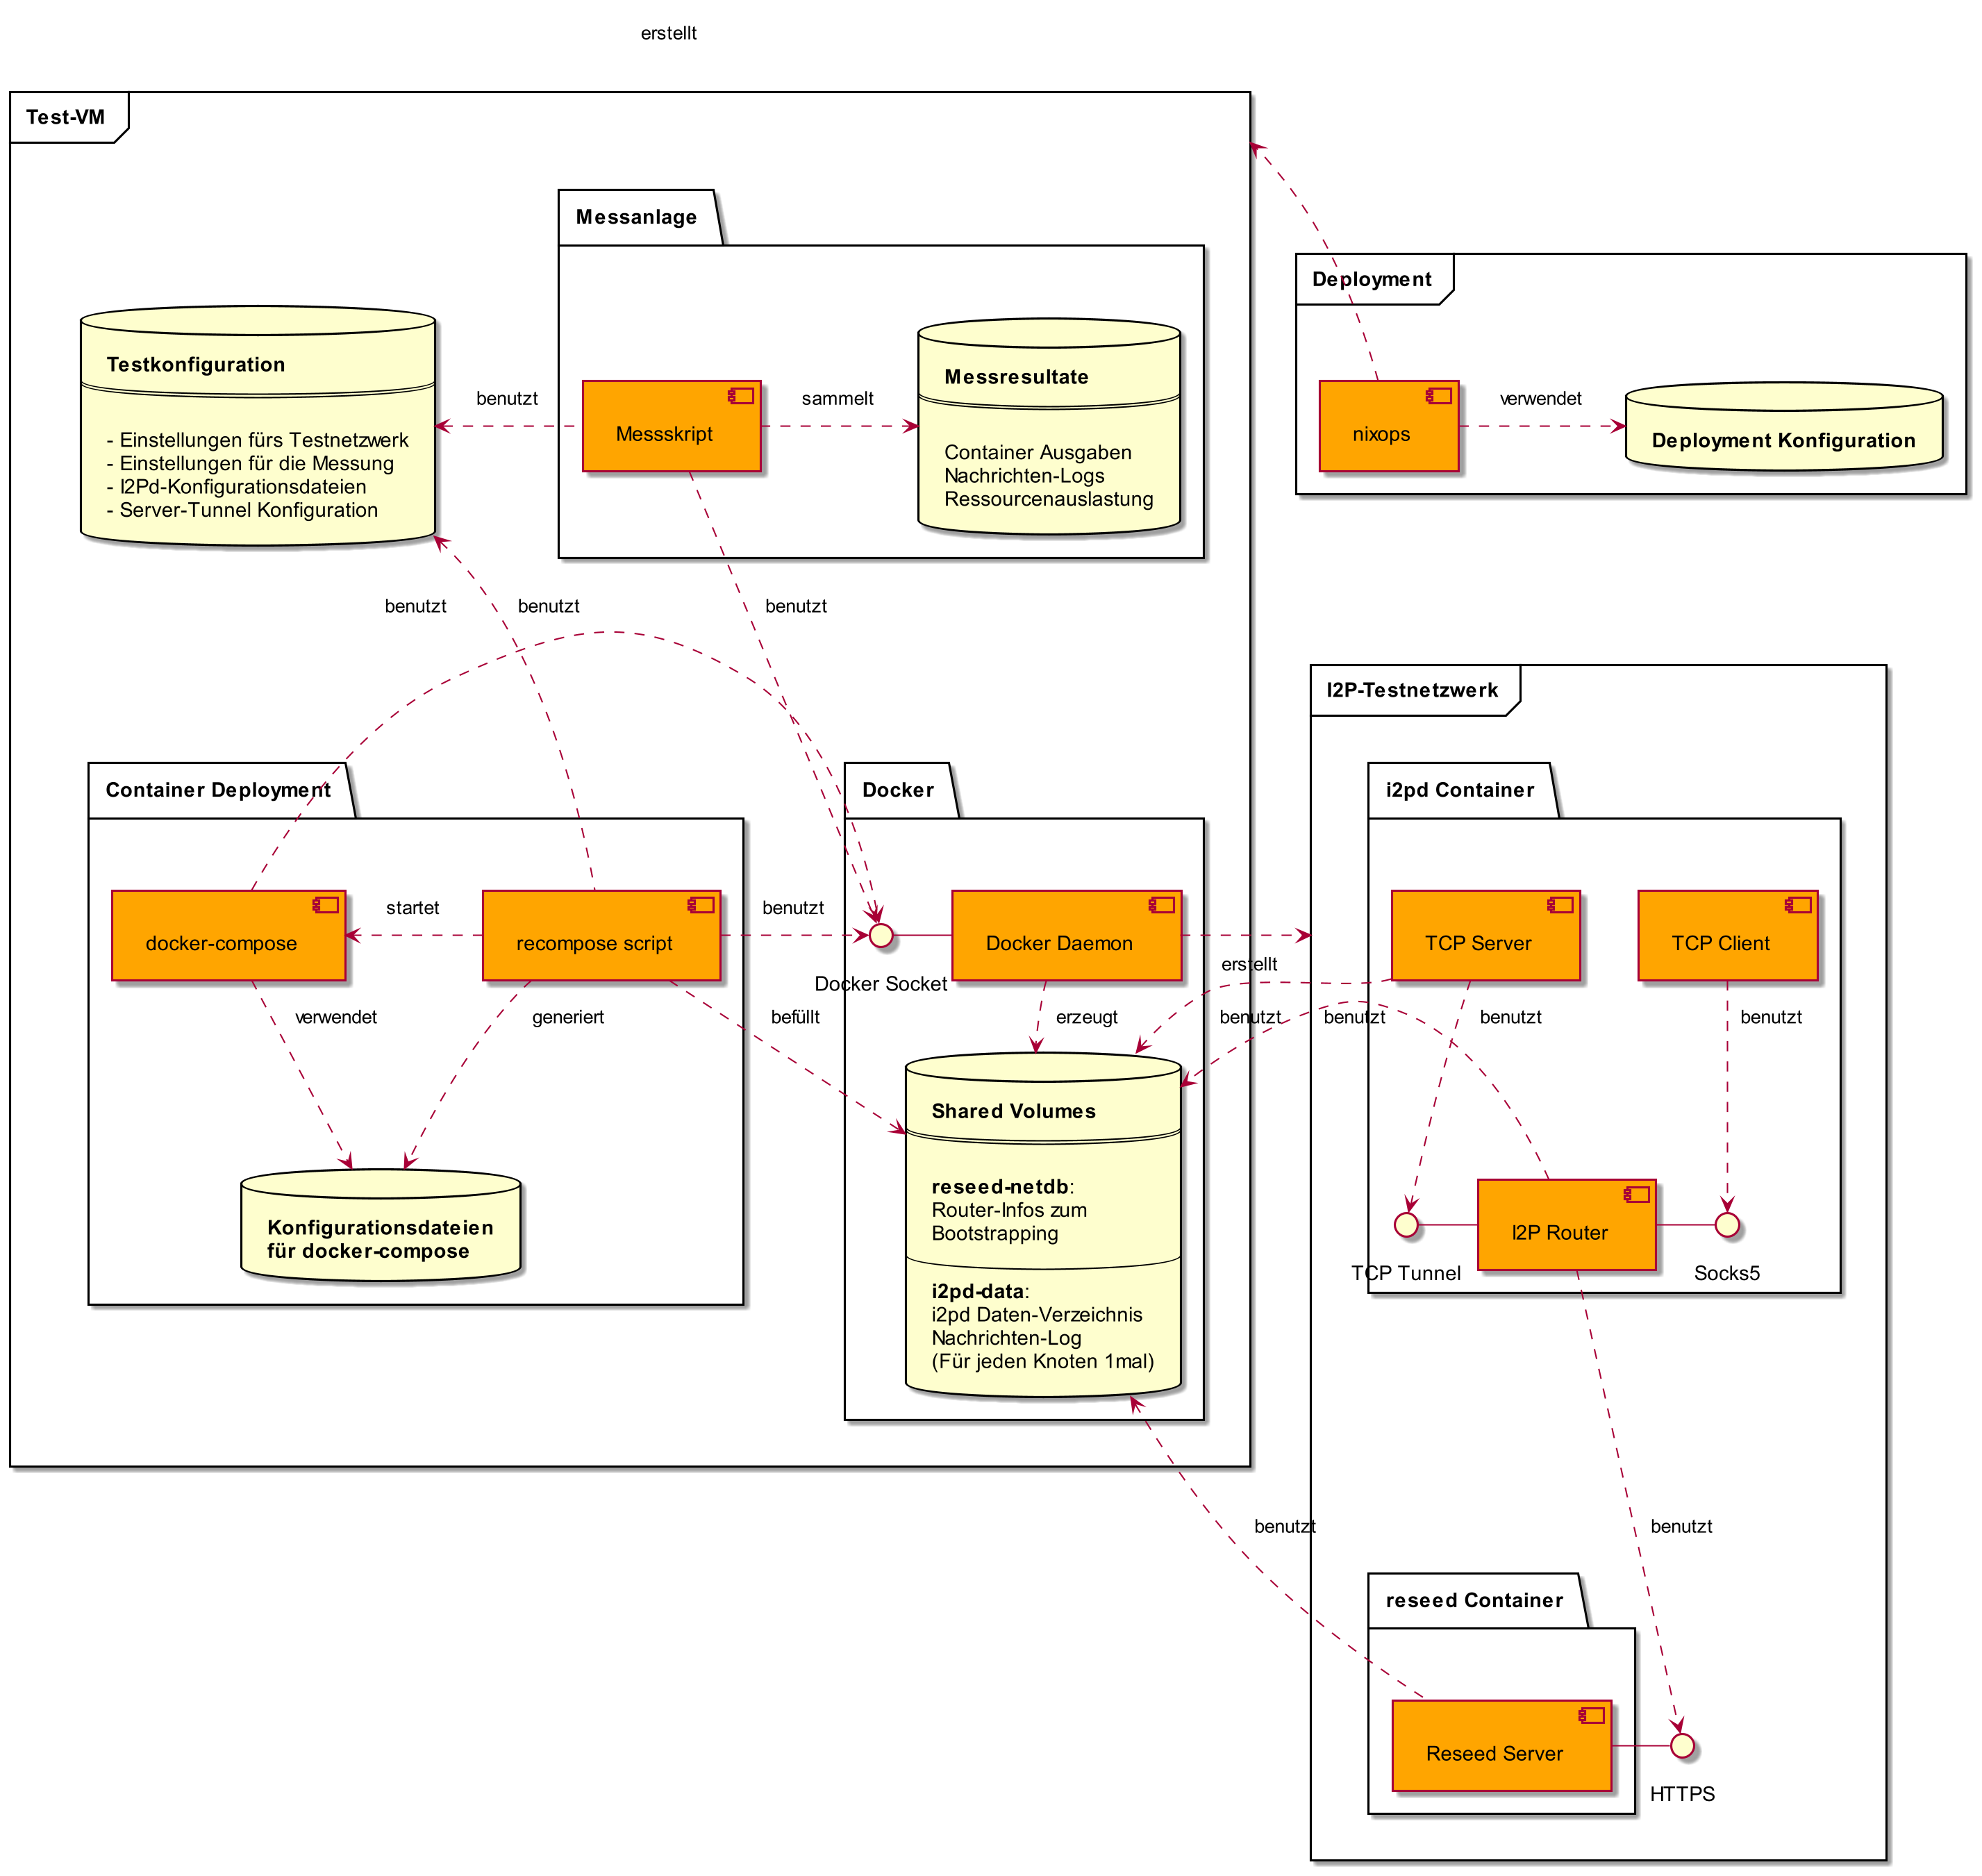
\includegraphics[width=1.1\textwidth]{include/uml/componentDiagram.png}
  \caption{Architektur-Diagramm}\label{fig:architektur-diagramm}
\end{figure*}


\section{Komponentendesign}\label{sec:komponentendesign}

In diesem Abschnitt werden die einzelnen Komponenten, wie dargestellt der Abbildung~\fullref{fig:architektur-diagramm}, genauer beschrieben.

\subsection{Deployment der Test-VM}

NixOps erlaubt es, mittels einer NixOS-Systemkonfiguration ein komplettes Linux auf diverse Arten von Maschinen zu deployen. Dies kann physische Hardware oder,
wie auch in diesem Falle, eine VM sein.
Somit sind alle benötigen Abhängigkeiten in Code-Form abgelegt und eine Test-VM kann reproduzierbar erstellt werden.

\subsection{Testkonfiguration}

Die Konfiguration des Teststands kann mittels einer JSON-Konfigurationsdatei einfach angepasst werden.
Da es sich hier um eine JSON-Datei handelt, kann diese falls nötig einfach von verschiedenen Programmen gelesen werden.
Einerseits wird diese vom Messkript gelesen, wie aber auch vom \lstinline|recompose| Skript.
Wie diese Konfiguration genau aussieht, wird im Abschnitt~\fullref{sec:konfigurationsoptionen} genauer erläutert.

\subsection{Recompose-Skript}

Das Recompose-Skript ist dafür verantwortlich das Docker-Netzwerk anhand der Konfiguration aufzubauen und zu verwalten.
Es ist das Kernstück der entwickelten Software.
Es handelt sich hierbei um einen Wrapper um Docker-compose.
Einerseits sorgt der Wrapper dafür, dass das Containernetzwerk korrekt aufgebaut wird (siehe Abschnitt~\fullref{sec:netzwerkisolation}) .
Andererseits generiert dieses die von Konfigurationsdateien für Docker-compose und managed die Shared-Volumes.
Docker-Compose erlaubt das automatisierte Erstellen und Abbauen von Netzwerken bestehend aus mehreren Docker-Containern.
Dazu liest Docker-compose jeweils eine oder mehrere YAML-Dateien.
In diesen YAML-Dateien können die verschiedenen Container, Netzwerke und Volumes und diverse Optionen deklariert werden, welche das zu erstellende Containernetzwerk beschreiben.
Im Benutzerhandbuch im Abschnitt~\fullref{sec:erstellen_des_testnetzwerks} wird kurz gezeigt, wie dieses Skript verwendet wird.

\subsection{i2pd-Container}

Hauptsächlich wird in diesem Container der \lstinline|i2pd|-Prozess ausgeführt.
Der TCP-Client und TCP-Server, welche zur Messung benötigt werden, sind ebenfalls direkt in diesem Container angesiedelt.
Diese sind in den Abschnitten \fullref{sec:tcpserver} und \fullref{sec:tcpclient} genauer beschrieben.
Dies verletzt zwar das Prinzip, dass man nur einen Prozess in einem Docker-Container ausführen sollte,
jedoch ist das Ziel, hiermit Messungenauigkeiten aufgrund eines zusätzlichen Containers zu vermeiden, sowie die Netzwerkkonfiguration zu vereinfachen.

\subsection{Reseed-Server}

Da das Testnetzwerk privat ist und somit nicht Teil des öffentlichen Netzwerks sein sollte \seereq{TISO}, wird ein Bootstrapping Prozess benötigt, da die öffentlichen Reseed-Server nicht erreichbar sind.
Dieser wurde so implementiert, das ein zusätzlicher Container im Testnetzwerk gestartet wird, welcher einen sogenannten Reseed-Server beinhaltet.
Die i2pd-Container fragen zu Beginn den Reseed-Server über HTTPS nach einer Liste von RouterInfos.
Dieser Ansatz hat den Vorteil, das so das Testnetzwerk schnell komplett neu aufgebaut und gestartet werden kann.
Weitere Details zum Bootstrapping-Vorgang sind im Abschnitt~\fullref{sec:umsetzung_bootstrap} zu finden.

\subsection{Messskript}

Das Messskript ist dafür verantwortlich, eine konfigurierte Anzahl an Nachrichten zur Latenzmessung durch das Testnetzwerk zu senden, damit Messdaten erstellt werden.
Die Nachrichten zur Latenzmessung werden vom TCP-Client eines zufälligen Knotens zum TCP-Server eines anderen zufälligen Knotens verschickt.
Somit kann sichergestellt werden, dass die Latenzmessungen repräsentativ sind für das gesamte Netzwerk.
Um das Netzwerk nicht zu überlasten, werden die Nachrichten sequentiell versendet und es wird nur eine Nachricht auf einmal versendet.
Zudem wird nach jeder versendeter Nachricht einige Sekunden (je nachdem was konfiguriert wurde) gewartet. Genaueres dazu im Abschnitt~\fullref{sec:messskript}.

\section{Umsetzung}\label{sec:umsetzung}

In folgendem Abschnitt wird nun beschrieben,
wie die im vorherigen Abschnitt aufgezeigte Systemarchitektur und das dazugehörige Komponentendesign effektiv umgesetzt wurde.
Zudem wird der Weg zur Lösung genauer beschrieben.
Zuerst wurde versucht ein I2P-Testnetzwerk unter Verwendung von NixOS-Containern zu erstellen (siehe Abschnitt \fullref{sec:la1_nixos}).
Jedoch wurde schlussendlich unter Verwendung von Docker-Compose eine andere Lösung gefunden, welche den Anforderungen gerecht wurde.
Der erzeugte Quellcode zur Erstellung des I2P-Testnetzwerk's sowie der Quellcode für die Messanlage ist im folgenden Repository zu finden:\\
\url{https://codeberg.org/mkuettel/i2p-testnet}

\section{Lösungsansatz: NixOS-VMs und NixOS-Container}\label{sec:la1_nixos}

Zu Beginn des Projekts wurde versucht, mit Hilfe von NixOps ein I2P-Testnetzwerk aufzubauen.
NixOps ist ein Tool zum Deployment von Netzwerken bestehend aus NixOS-Maschinen.
NixOS ist eine Linux-Distribution basierend auf dem Paket-Manager Nix,
der es erlaubt es reproduzierbare Softwarepakete zu erzeugen.
Er kann mit einer deklarativen und funktionalen Programmiersprache konfiguriert werden\footnote{Siehe die Webseite von NixOS für weiterführende Informationen: \url{https://nixos.org}}.
Dieser Ansatz wurde zu Beginn aus mehreren Gründen ausgewählt.
Einerseits setze ich auch selber NixOS seit mehreren Jahren ein und NixOps ist somit das dazugehörige Deployment-Tool.
Andererseits legt Nix enormen Wert auf Reproduzierbarkeit.
Das gesamte Netzwerk bis hin zum OS könnte anhand einer Nix-Konfiguration wiedererstellt werden.
Auch könnten Konfigurationen für I2P-Knoten wiederverwendet werden, egal ob diese nun in Container,
VMs oder auf echter Hardware deployed werden.
Dies ist möglich da, System-Konfigurationen oder Teile davon bei NixOS unabhängig von der Konfiguration der effektiven Infrastruktur sind.
Angefangen wurde damit, dass mit NixOps ein Netzwerk bestehend aus einer einzelnen VirtualBox-VM erstellt wurde.
Anschliessend wurden mehrere I2P-Knoten als NixOS-Container innerhalb dieser VM zu erstellt und es wurde versucht eine Lösung für das Bootstrapping Problem zu finden.
Jedoch ist man mit diesem Ansatz immer wieder an verschiedenen Stellen auf Probleme gestossen:

\begin{itemize}
    \item \textbf{Netzwerkkonfiguration:} Die Knoten konnten nicht korrekt untereinander kommunizieren. Es war nicht möglich einen anderen Container mittels eines \lstinline|ping|-Befehls zu erreichen.
        Es hat sich herausgestellt, dass das Routing zwischen den Containern sowie die Netzwerkmasken nicht korrekt konfiguriert wurden und es keine Option gab,
        diese Routen innerhalb der Nix-Deklaration richtig zu setzen.
        Aufgrund dessen wurde das NixOS-Modul für NixOS-Container erst angepasst.
        Somit konnte man die Routing-Probleme beheben und Optionen hinzufügen, um die Netzwerkmasken der Knoten korrekt zu setzen. %TODO: reference commit
        Das NixOS-Container Modul sc erstelltheint also nicht ausgereift zu sein.
    \item \textbf{Docker-Kompatibilität:} Auch hat man versucht anstatt von NixOS-Containern, Docker-Container auf NixOS zu erstellen.
        Dies hätte es erlaubt, die bestehenden Container von DIVA.EXCHANGE wiederzuverwenden.
        Jedoch schien der Support für Docker auch nicht ausgereift genug zu sein.
        Man konnte auf meinem Laptop keine Docker-Images bauen für das Testnetzwerk, da dies libvirt/QEMU-Support benötigt.
        Dies war unter gleichzeitiger Verwendung von VirutalBox nicht möglich, da nur ein Hypervisor gleichzeitig ausgeführt werden kann.
        Man hat auch versucht den Hypervisor auf libvirt/QEMU zu wechseln, was aber schon am Deployment der VM scheiterte.
    \item \textbf{Skalierungsprobleme:} Während dem Entwickeln hat man jeweils 2 oder 8 Knoten auf einmal erstellt, um schnell ein Feedback zu erhalten.
        Um den Reseeder zu testen hat man jedoch versucht 103 Knoten auf einmal zu erstellen.
        Jedoch hat nur schon das Generieren und Auswerten der NixOS-Systemkonfigurationen für alle diese NixOS-Container extrem viel Arbeitsspeicher benötigt.
        Meine 16 GB Arbeitsspeicher in meinem Laptop waren nach mehreren Sekunden gefüllt.
        Man konnte somit die Knoten nicht einmal erstellen und deployen, da nur schon das berechnen der NixOS-Systemkonfigurationen zu ineffizent implementiert ist.
\end{itemize}
Somit war klar das dieser Lösungsansatz nicht funktionieren konnte und es musste ein grundsätzlich anderer Ansatz zur Erstellung der Container gefunden werden.

\section{Lösung mit Docker-Compose}

Nachdem sich herausgestellt hat, dass der Lösungsansatz mit NixOS-Containern nicht funktioniert, wurde eine Container-Orchestration Lösung gesucht.
Um unnötige Komplexität zu vermeiden wurde auf das einfachere Tool Docker-compose gesetzt.
Zudem hat der Auftraggeber bereits Erfahrungen mit diesem Tool gemacht und es auch schon eingesetzt um i2pd-Netzwerke zu erstellen
für die Entwicklung an der DIVA-Blockchain.
Anhand der \lstinline|docker-compose.yml|-Datei vom Auftraggeber,
konnte ein kleines öffentliches I2P-Testnetzwerk mit acht festkodierten i2pd-Container werden.
Dies wurde anschliessend als Ausgangspunkt verwendet.

\subsection{Skalierung}\label{sec:scaling}

Damit verschiedene Anzahl an I2P-Knoten im privaten Testnetzwerk getestet werden können, müssen diese skaliert werden können.
Anfangs wurde versucht auf die Skalierungsfunktion von Docker-compose zurückzugreifen.
Mittels der \lstinline|--scale|-Option des \lstinline|docker-compose up| Befehls, können aus einem einzigen deklarierten Container mehrere Container instanziiert werden. Man kann diesen also nur einmal definieren, wie aufgezeigt in folgendem Listing:
\begin{lstlisting}{language=yaml}
# ... 
services:
  i2pd:
    build:
      context: "./docker/i2p"
    environment:
      ENABLE_TUNNELS: 1
    networks:
      i2ptestnet:
        ipv4_address: "10.23.128.1"
# ...  
\end{lstlisting}

Jedoch bin ich mit diesem Ansatz auf Netzwerkprobleme gestossen,
sodass die \lstinline|i2pd|-Container nie untereinander direkt kommunizieren konnten.
Die Vermutung besteht, dass diese Skalierungsfunktion nicht für P2P-Netzwerke geeignet ist,
denn im Normalfall wird sie wohl verwendet einen Service auf einem Tier zu skalieren.
Beispielsweise können damit Datenbank- oder Webserverinstanzen skaliert werden, die aber natürlich normalerweise nie untereinander kommunizieren müssen.
Auch scheint die \lstinline|--scale|-Option veraltet zu sein und wird durch neuere Features wie \lstinline|docker swarm| ersetzt.
Dieses Problem wurde schlussendlich so gelöst,
dass nun dynamisch für jeden zu erstellenden Knoten eine \lstinline|i2pd|-Container-Deklaration anhand eines JSON-Templates generiert wird.
Dieses JSON-Template ist in \lstinline|docker/i2p-node-base.json| zu finden.
Die fehlenden Werte, so wie z.B. eine statische IP, werden beim ausführen des Recompose-Skripts ausgefüllt.
Anschliessend werden die verschiedenen Deklarationen zusammengeführt und in eine generierte \lstinline|docker-compose.yml|-Datei abgelegt.
Dies funktionierte sehr gut da, YAML ein Superset von JSON ist. Vereinfacht gesagt: Jede JSON-Datei ist auch eine gültige YAML-Datei.

Im folgenden Quellcodelisting sind die beiden relevanten Funktionen aus der Datei \lstinline|lib/compose.bash| aufgezeigt.
Die Funktion \lstinline|generate_node_config| erstellt aus dem JSON-Template eine einzelne Service Konfiguration.
Insbesondere werden in Zeile 69 die fehlenden Felder im JSON-Template ausgefüllt.
Die Funktion \lstinline|generate_all_node_configs| erstellt die Datei,
die dann anschliessend von Docker-compose eingelesen werden kann.

\begin{lstlisting}[firstnumber=61]{language=bash}
generate_node_config() {
    local id="$1"
    local i2pd_config_file="$2"
    local segment3=$((id / 256 + 128))
    local segment4=$((id % 256))

    local nodefile="$(mktemp)"

    jq  --arg ipv4_address "10.23.${segment3}.${segment4}" \
        --arg name "\${COMPOSE_PROJECT_NAME}_i2pd_$id" \
        --arg volume_dir "./docker/volumes/i2pd-data-$1:/home/i2pd/data" \
        --arg confarg "i2pd_config_file=$i2pd_config_file" \
        --arg bandwidth "$(get_bandwidth "$id")" \
        ' .container_name = $name
        | .networks["i2ptestnet"]["ipv4_address"] = $ipv4_address
        | .volumes += [$volume_dir]
        | .build.args += [$confarg]
        | .environment["BANDWIDTH"] = $bandwidth
        ' \
        < "$base_dir"/docker/i2p-node-base.json \
        > "$nodefile"

    if [[ "$(getconf network.private)" == "true" ]]; then
        jq  --arg reseed_wait_url "http://$RESEED_IP:8443/i2pseeds.su3" \
            '.environment["RESEED_WAIT_URL"] = $reseed_wait_url' \
            < "$nodefile" \
            | sponge "$nodefile"
    fi

    jq --arg i $1 '{("i2pd_" + $i): .}' < "$nodefile"
    rm "$nodefile"
}

generate_all_node_configs() {
    local amount="$1"
    local i2pd_config_file="$2"

    (
        for i in $(seq 1 "$amount"); do
            generate_node_config "$i" "$i2pd_config_file"
        done
    )   | jq -s 'add | {"version": "3.8", "services": .}'
}
\end{lstlisting}

Da hiermit pro Knoten eine statische IP pro Container vergeben wird,
konnte mit dieser Lösung nicht nur das Skalierungsproblem, sondern auch die Netzwerkprobleme gelöst werden.
Die konfigurierte Anzahl an Containern können nun direkt miteinander kommunizieren.

Die Skalierung auf 128 Knoten auf einem einzelnen Rechner hat sich als weiteres Problem herauskristallisiert,
dass die Knoten nicht miteinander kommunizieren können.
Nach einer Fehleranalyse hat sich herausgestellt, dass die ARP-Neighbor-Tabelle der
Test-VM überlaufen war.
Dies ist geschehen, da sich die Container eine einzelne ARP-Neighbor-Tabelle teilen, nämlich die des Hosts.
Als Lösung wurden die ARP-Neighbor-Tabelle des Hosts einfach vergrössert.
Aus diesem Grund wurde ein zusätzliches Skript erstellt, welches Root-Rechte benötigt, da ein \lstinline|sysctl|-Befehl gebraucht wird um die Linux-Kernel-Parameter umzustellen.
Hier der relevante Ausschnitt aus \lstinline|bin/networking-sysctls|, der die Grösse der ARP-Neighbor-Tabelle erhöht, abhängig von der konfigurierten Anzahl an Knoten:
\begin{lstlisting}[firstnumber=9]{language=bash}
num_nodes="$(getconf 'nodes.amount')"

arp_table_size=$((num_nodes * num_nodes))

sysctl net.ipv4.neigh.default.gc_thresh1=$arp_table_size
sysctl net.ipv4.neigh.default.gc_thresh2=$((arp_table_size * 2))
sysctl net.ipv4.neigh.default.gc_thresh3=$((arp_table_size * 2))
\end{lstlisting}

\subsection{Bootstrapping und Reseed-Server}\label{sec:umsetzung_bootstrap}

Die \lstinline|i2pd|-Implementation beinhaltet selber keinen Reseed-Server, sondern es ist eine zusätzliche Software ist vonnöten.  
Die Go-Implementation dieses Reseed-Servers ist hier in meinem Repository zu finden:\\ \url{https://codeberg.org/mkuettel/i2p-tools}\\
Diese basiert auf der Implementation die auch von DIVA.EXCHANGE verwendet wird:\\ \url{https://codeberg.org/diva.exchange/i2p-tools}\\
Welche schlussendlich wiederum auf der folgenden Implementation auf GitHub basiert:\\  \url{https://github.com/MDrollette/i2p-tools}\\

Die Implementation aus meinem eigenen Repository wurde insofern angepasst,
dass alle verfügbaren RouterInfos verwendet werden. Standardmässig werden nur 75 \% davon überhaupt verwendet und bei einer Anfrage an die Knoten abgeliefert.
Der Grund dafür ist leider unbekannt, jedoch macht dies für meinen Anwendungszweck im Testnetzwerk keinen Sinn. 
Man braucht so nur unnötig mehr Knoten um das Netzwerk aufstarten zu können.
Deshalb wurden ich auch die Anzahl an RouterInfo-Dateien und die Anzahl an verschiedenen SU3-Dateien mit einem verschiedener Liste von RouterInfo--Dateien konfigurierbar gemacht.
Die Konfiguration dieser Optionen kann eine wichtige Rolle spielen, denn diese bestimmen  die Liste an Peers die den I2P-Routern geliefert beim Start geliefert werden und somit den Konnektivitätsgrad der Knoten.

\subsubsection{Ablauf}

Der Bootstrapping-Vorgang im Testnetzwerk wird wie folgt abgehandelt (vgl. Abbildung~\fullref{fig:bootstrap-diagram}):

\begin{enumerate}
    \item Erstellen der Container für den Reseed-Sever und den I2P-Knoten
    \item Der Reseed-Server erstellt die nötigen Schlüssel und Zertifikate, um einerseits später den HTTPS-Reseed-Server zu starten und andererseits die SU3-Dateien zu signieren.
    \item Der Reseed-Server-Container fängt an zu warten bis er alle RouterInfo's von allen I2P-Knoten erhalten hat, die im Hintergrund vom Recompose-Skript gesammelt werden.
    \item Die I2P-Router werden kurzzeitig gestartet, bis sie Ihre RouterInfo Datei erstellen. Die I2P-Router werden anschliessend wieder gestoppt, da der Reseed-Server im Moment noch nicht in Betrieb ist, da ihm die RouterInfos noch fehlen.
    \item Die I2P-Knoten-Container warten anschliessend, bis der HTTPS-Reseed-Server verfügbar ist.
    \item Auf der Test-VM kopiert ein Hintergrund-Job alle RouterInfos vom I2P-Container in die NetDb des Reseed-Server-Containers.
    \item Nach kurzer Zeit hat der Reseed-Server-Container alle benötigten RouterInfos. Nun generiert dieser die SU3-Datei aus den RouterInfos und startet anschliessend effektiv den HTTPS-Reseed-Server.
    \item Die I2P-Knoten-Container können nun den HTTPS-Reseed-Server erreichen und somit wird der I2P-Router gestartet.
    \item Die I2P-Router laden die SU3-Datei herunter und können so die anderen Knoten ausfindig machen und Ihre Arbeit starten.
\end{enumerate}

Welche Reseed-Server ein I2P-Router anfragt, kann in der \lstinline|i2pd.conf| mittels der Konfigurationsoption \lstinline|urls| festgelegt werden.

\begin{landscape}% Landscape page
\begin{figure*}[ht]
  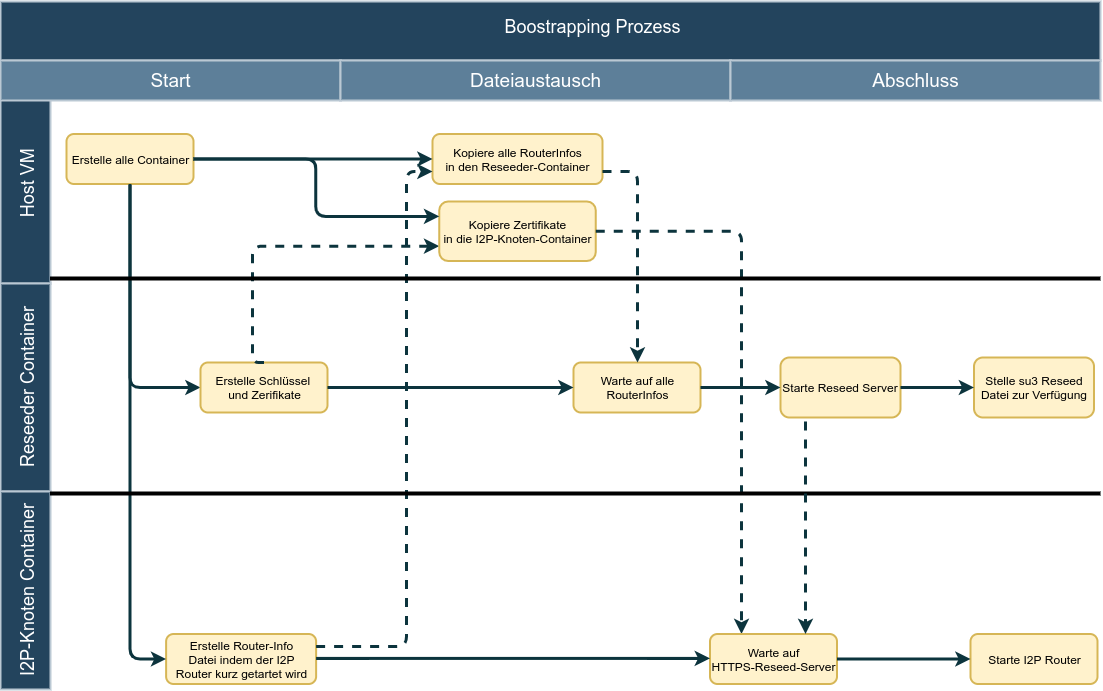
\includegraphics[height=0.85\textwidth]{bootstrap-diagram.png}
  \caption{Der Bootstrapping-Vorgang}\label{fig:bootstrap-diagram}
\end{figure*}
\end{landscape}% Landscape page

\subsection{Konfigurationsoptionen}\label{sec:konfigurationsoptionen}

Diverse Konfigurationsoptionen wurden implementiert um verschiedene Tests durchführen zu können und werden in der JSON-Datei \lstinline|config.json| im I2P-Testnet Repository abgelegt.
Jede der Optionen ist ein Schlüssel in der JSON-Datei und ist in der folgenden Auflistung kurz beschrieben:

\begin{itemize}
    \item Netzwerk-Optionen (\lstinline|network|):
        \begin{itemize}
        \item \lstinline|name|: Name des Docker-Netzwerks.
        \item \lstinline|private|: Wird auf \lstinline|true| gesetzt, wenn es sich um ein privates Testnetzwerk handeln soll. Die Einstellung \lstinline|false|, um dem öffentlichen I2P-Netzwerk beizutreten, wurde nicht komplett implementiert und nicht getestet.
        \end{itemize}
    \item Reseeder-Optionen (\lstinline|reseeder|):
        \begin{itemize}
        \item \lstinline|num_router_infos_per_node|: Anzahl RouterInfos pro SU3-Datei. So viele Peers kennt ein Knoten beim Start des Netzwerks.
        \item \lstinline|num_different_seed_files|: Anzahl Verschiedene SU3-Dateien. Der Reseed-Server wählt so viele verschiedene randomisierte Sets an RouterInfos aus.
        \end{itemize}
    \item Knoten-Optionen (\lstinline|nodes|):
        \begin{itemize}
        \item \lstinline|amount|: Anzahl Knoten im Testnetzwerk. Diese Option bestimmt wie viele i2pd-Knoten ins Testnetzwerk eingebunden werden.
        \item \lstinline|config_file|: Relativer Pfad zur i2pd-Konfigurationsdatei (\lstinline|i2pd.conf|) für alle Knoten. Darin können alle \lstinline|i2pd|-Optionen gesetzt werden (z.B. Tunnellänge, Netzwerk-ID, etc.).
        \item \lstinline|bandwidth|: Eine Liste von Zahlen. Dabei stellt jede Zahl eine Bandbreitenlimite (in kB) eines einzelnen Knotens dar. Das heisst die erste Zahl ist die Bandbreitenlimit des ersten Knotens, die zweite Zahl die Bandbreitenlimite des zweiten Knotens, usw. Sind zu wenige Zahlen in der Liste verfügbar wird wieder von Vorne angefangen. Wird nur eine Liste mit einer Zahl angegeben, so gilt dies also für alle Knoten.
        \end{itemize}
    \item Mess-Optionen (\lstinline|measurement|):
        \begin{itemize}
        \item \lstinline|message_size_kb|: Nachrichtengrösse (in kB).
        \item \lstinline|num_messages|: Anzahl an sequentiellen Nachrichten die versandt werden. 
        \item \lstinline|sleep_interval|: Wartezeit in Sekunden zwischen zwei sequentiellen Nachrichten.
        \end{itemize}
\end{itemize}

Eine Beispiel \lstinline|config.json| könnte zum Beispiel so aussehen.

\begin{lstlisting}{language=json}
{
    "network": {
        "name":"network.i2pd.local",
        "private": true
    },
    "reseeder": {
        "router_infos_per_node": 48,
        "num_different_seed_files": 64
    },
    "nodes": {
        "amount": 64,
        "config_file": "conf/i2pd.org.conf",
        "bandwidth": [1000000]
    },
    "measurement": {
        "message_size_kb": 16,
        "num_messages": 1024,
        "sleep_interval": 6
    }
}
\end{lstlisting}

\subsection{Netzwerkisolation}\label{sec:netzwerkisolation}

Während unserer Tests wollen wir nur Traffic unserer eigenen Knoten im Netzwerk und äussere Einflüsse vermeiden.
Dies, um bestmögliche und unbeeinflusste Messungen tätigen zu können.
Docker-compose respektive Docker bietet eine Option, ein internes Netzwerk zu erstellen,
welches einerseits vom Host nicht direkt erreichbar ist
und zudem die Container nicht auf das Host-Netzwerk zugreifen können.
Das folgende Quellcodelisting zeigt den Abschnitt für die Netzwerkkonfiguration wie deklariert in der \lstinline|docker-compose.yml|.
Wichtig sind hier die Optionen \lstinline|driver: bridge| und \lstinline|internal: true|, die ein internes Docker-Netzwerk erstellen.
Die zusätzliche Option \lstinline|enable_icc| stellt sicher, das die Container jedoch untereinander kommunizieren können.
\begin{lstlisting}{language=yaml}
networks:
  i2ptestnet:
    name: $NETWORK_NAME
    driver: bridge
    internal: true
    driver_opts:
      com.docker.network.bridge.enable_icc: "true"
      com.docker.network.bridge.enable_ip_masquerade: "true"
    ipam:
      driver: default
      config:
        - subnet: 10.23.0.0/16
\end{lstlisting}

Zusätzliche Optionen zur Abgrenzung vom öffentlichen I2P-Netzwerk können in der \lstinline|i2pd.conf| spezifiziert werden.
Einerseits gibt es die Option \lstinline|netid|; diese ist standardmässig auf die Nummer 2 gesetzt, da dies die Netzwerk-Id des öffentlichen I2P-Netzwerks ist.
Diese Option ist im Testnetzwerk jedoch zur Abgrenzung auf die Nummer 23 gesetzt. 
I2P-Router mit einer anderen Netzwerk-ID werden nie miteinander kommunizieren.
Für Tests mit dem öffentlichen Netzwerk gäbe es zusätzlich noch die Option \lstinline|family| \parencite{noauthor_family_nodate}.

\subsection{Adressbuch}

Standardmässig wird jeder Destination eine b32-Adresse gegeben.
Diese ist jedoch nicht einfach zu handhaben und stattdessen ist es einfacher, die Knoten direkt anhand ihrer Nummer zu adressieren.
Diese Adressen werden dann automatisch vom Socks5-Proxy, der \lstinline|i2pd| mitliefert aufgelöst.
Damit kann das Messskript vereinfacht werden, da es dann nicht die genauen Adressen zusammensuchen muss.

Auch wird die Auswertung damit vereinfacht, weil der TCP-Client den verwendeten Namen des TCP-Servers auch in die Nachricht hineinpackt und der TCP-Server diesen als Messausgabe abspeichert.
Es wird beim Startvorgang des Netzwerks für jede erstellte Destination für den TCP-Server ein Adressbucheintrag erstellt.
Dieses Adressbuch ist eine einfache CSV-Datei wird ebenfalls im Bootstrapvorgang an alle Knoten verteilt.
Im Falle von acht Knoten im Netzwerk sieht diese Datei beispielsweise so aus:

\begin{lstlisting}[numbers=none]
tcpsrv-1.i2p,b2cdodoyqg5v6go56bkaevvw777e2wyiflqh6zyyyxugy4cqlzuq
tcpsrv-2.i2p,r6axddltht76mrtp5lrxtdxncilhgp7bcajkqtsj7l7fmoebgs3a
tcpsrv-3.i2p,ddhznqpxtgac7qa6yg6uzfpd55xoa2zfc4dwg4rh4qucx7veswlq
tcpsrv-4.i2p,3tyncnh7j4akqirrbdi4ek7nlysqmuvyav3ix326vwixvgoviz3q
tcpsrv-5.i2p,xj3qduyqur54v3mjgsxn6xa56q2ojyysf5n3bonpxyfxy5trnoja
tcpsrv-6.i2p,pt64eojrsvrp5w5izgwlide7j6vuw5td6g2pfrkurwsnmb4i7q2q
tcpsrv-7.i2p,aat6wqge3o7k2nabpwxrcu2vbbiydf3mj6n5k2zrrtozkrrpyfoa
tcpsrv-8.i2p,4wm4pqautqqb3a6yw3xif4zgwwu4v5tvpwv6onha27p5pkcqqepq
\end{lstlisting}

In der ersten Spalte ist der vereinfachte Name angegeben und in der zweiten Spalte die b32-Adresse, jedoch ohne die Endung \lstinline|.i2p|.


\subsection{TCP-Server}\label{sec:tcpserver}

Für Tests am Anfang wurde das Tool Netcat verwendet.
Dies hat gut funktioniert, um die Konnektivität im Netzwerk zu testen,
hat aber zur effektiven Messung nicht funktioniert, da es nicht geklappt hat die TCP-Verbindung nachdem eine Nachricht erhalten wurde zu schliessen, was dazu führte, das dass Messskript stecken blieb.
Auch erlaubt es Netcat nicht mehrere TCP-Verbindungen anzunehmen und die Verbindungen korrekt zu schliessen.
Deshalb wurde eine \lstinline|epoll|-basierte C-Implementation eines TCP-Servers erstellt, um die komplette Kontrolle über den Netzwerksocket zu bekommen.
Dies erlaubt es die Latenz genauer zu messen und auch den TCP-Verbindungsaufbau nicht mitzumessen, sowie die Nachrichtenübermittlung auf Socket-Ebene kontrollieren zu können.
Somit konnte die TCP-Verbindung nach Erhalt einer Nachricht korrekt geschlossen werden.
Auch wurde C und nicht z.B. Python gewählt, um den Arbeitsspeicher und CPU-Gebrauch der Containers so tief wie möglich zu halten.
Die Implementation des TCP-Servers ist in der Datei \lstinline|docker/i2p/messenger/epoll-server.c| zu finden.

\subsubsection{TCP-Server Tunnel}

Diese Tunnel-Konfiguration führt dazu, dass I2P eine neue Destination mit einer .b32-Adresse erstellt, damit der TCP-Server innerhalb des I2P-Netzwerks erreicht werden kann.
Mit der folgenden Tunnel-Konfigurations-Datei wird der \lstinline|i2pd| konfiguriert, um einen TCP-Server-Tunnel zur Verfügung zu stellen:
\begin{lstlisting}
# serve some tcp service to others in the network
[tcp-in]
type = server
host = 127.0.0.1
port = 2323
keys = tcp-in.dat
gzip = false
enableuniquellocal = true
\end{lstlisting}

Hierbei gilt es zu beachten, dass die Schlüssel für die Destination, angegeben mit der \lstinline|keys|-Option, beim Aufstarten generiert werden.
Auch wurde mittels der Option \lstinline|gzip| die Komprimierung deaktiviert, damit auch wirklich die richtigen Nachrichten-Grössen übermittelt werden.
Die Option \lstinline|enableuniquellocal| wurde ursprünglich aktiviert, um die Auswertung zu vereinfachen. Denn diese führt dazu das der TCP-Server nicht immer dieselbe Ausgangsadresse \lstinline|127.0.0.1| bekommt, sondern je nach Sender der Nachricht eine andere \lstinline|127.0.0.0/8|-Adresse anhand der ersten Bytes des Public-Keys erhält. Jedoch wurde schlussendlich nicht auf diese Möglichkeit die Knoten zu identifizieren zurückgegriffen, da die Knoten einfacher mithilfe des Adressbuch identifiziert werden konnten.

\subsection{TCP-Client}\label{sec:tcpclient}

Damit der TCP-Client sich mit dem I2P-Overlaynetzwerk verbinden kann, muss er fähig sein mit einem Socks5-Proxy zu kommunizieren.
Zudem gilt es den Socks5-Proxy richtig zu konfigurieren,
denn die Namensauflösung muss auch über das I2P-Netzwerk abgehandelt werden.
Nur so können die b32-Adressen aufgelöst werden, sofern diese im Adressbuch vorhanden ist.
Anhand einer \lstinline|.b32.i2p|-Adresse kann die NetDB nach einem zugehörigen LeaseSet abgefragt werden, welches Zugriff auf die gewünschte Destination bietet.
Der TCP-Client ist ein kleines C-Programm, welches in der 
in der Datei \lstinline|docker/i2p/messenger/client.c| zu finden ist.
Zusammengefasst macht es nichts anderes als
eine Verbindung mit einem Socks5-Proxy aufzubauen, und eine TCP-Nachricht der definierten Grösse mit ein durch den Proxy an die richtige Destination zu versenden.
Wie diese Nachricht aufgebaut ist wird im Abschnitt~\fillref{sec:nachricht_latenzmessung} genauer erläutert.
Das TCP-Client Programm bietet folgende Kommandozeilen-Optionen:

\begin{lstlisting}
Usage:  messenger [-h] [-S proxy_server] [-P proxy_port] [-d destination] [-p dest_port]
Parameters:
  -h                    display command line help
  -S proxy_server       proxy server host name or IP address
  -P proxy_port         proxy port number
  -d destination        he hostname or ip of the server connected through the proxy
  -p dest_port          destination port number
  -m messagesize        size of the message to send in Kb
  -o originator         an identifier for the originator of the message
  -v                    verbose mode
  -d                    debug mode (overrides -v)
Description:
This client is used to send messages to measure the latency of the i2p network
\end{lstlisting}

\subsubsection{Socks5-Proxy für den TCP-Client}

Dieser Socks5-Proxy ist der Gateway um mit dem I2P-Overlaynetzwerk zu kommunizieren.
Der folgende Ausschnitt aus der \lstinline|i2pd.conf| zeigt auf wie der Socks5-Proxy konfiguriert wurde:

\begin{lstlisting}
[socksproxy]
## Uncomment and set to 'false' to disable SOCKS Proxy
enabled = true
## Address and port service will listen on, like 127.0.0.1
address = 127.0.0.1
port = 4445
\end{lstlisting}

Zusätzlich könnte in diesem Abschnitt auch die Länge der Tunnels bestimmt.

\subsection{Nachricht zur Latenzmessung}\label{sec:nachricht_latenzmessung}

Die darüberliegende Blockchain-Schicht von DIVA.EXCHANGE versendet mittels eines Gossip-Protokolls die neuen Blocks der Blockchain an alle Knoten.
%TODO: add gossip protocol to glossary
Diese 64KB grossen Blocks werden über eine Web-Socket-Verbindung an die Nachbarknoten übermittelt.
Die Nachbarknoten leiten diese dann wiederum an ihre jeweiligen Nachbarknoten weiter.
Dieser Prozess wird solange wiederholt bis alle Knoten im Netzwerk den neuen Block erhalten haben.
Nach Absprache mit dem Auftraggeber wird dies im Testnetzwerk mittels versenden von TCP-Nachrichten nachgestellt.
Bei Web-Sockets handelt es sich vereinfacht ausgedrückt wiederum um eine TCP-ähnliche Verbindung über HTTP. Zudem verwendet HTTP auch TCP auch als Transportschicht.

Eine Nachricht welche vom TCP-Client zum Server übermittelt wird, besteht aus folgenden Elementen:

\begin{itemize}
    \item Zufällige Daten (standardmässig 64KB, konfigurierbar)
    \item Knoten Nummer des Senders
    \item Destination-Adresse des Empfängers vom Adressbuch (beinhaltet auch die Knoten Nummer des Empfängers)
    \item Grösse der versendeten Nachricht in Bytes (standardmässig 63255)
    \item Versandzeitpunkt in Nanosekunden seit dem 1.1.1970
    \item Empfangszeitpunkt in Nanosekunden seit dem 1.1.1970
\end{itemize}

Der TCP-Server legt alle erhaltenen Nachrichten im I2P-Container in einem Nachrichten-Log ab.

\subsection{Das Messskript}\label{sec:messskript}

Die Nachrichten zur Latenzmessung werden versendet unter Verwendung des \lstinline|docker exec|-Befehls.
Damit wird innerhalb des zufällig ausgewählten i2pd-Containers ein TCP-Client-Prozess gestartet.
Dieser verbindet dann auf den Socks5-Proxy im gleichen Container.
Anschliessend schickt der TCP-Client die Nachricht der gewählten Grösse ins I2P Netzwerk.

Bevor das Messskript gestartet werden kann, müssen jedoch einige Bedingungen erfüllt werden.
Erstens muss mittels dem Recompose-Skript das Testnetzwerk in Betrieb genommen werden.
Zweitens muss gewartet werden, bis der Bootstrapping-Vorgang im Testnetzwerk abgeschlossen wurde.
Zu guter Letzt muss noch einige Zeit gewartet werden und sichergestellt werden, dass das Netzwerk bereit ist und die Exploratory-Tunnels aufgebaut sind.
Dies ist um sicherzustellen, dass keine Messungenauigkeiten auftreten.
Einerseits gehen so keine Messpakete verloren, andererseits könnten die Latenzmessungen verfälscht werden, wenn die Tunnels erst noch aufgebaut werden müssen.
Das Messskript ist in der Repository in der Datei \lstinline|bin/measure-message-latency| zu finden.

\section{Testing}

Da ein gesamtes Netzwerk simuliert wurde mit dynamisch vielen Containern, konnte nicht automatisch unter Verwendung von \glstext{ci} getestet werden.
Viele \glsname{CI} Lösungen (wie zum Beispiel das angebotene GitLab im EnterpriseLab der HSLU) verwenden eine andere Syntax zur Definition von Containern als Docker-compose und die definierten Container lassen sich nicht skalieren.
Somit musste oft auf manuelles Testen zurückgegriffen werden.
Jedoch hat sich während des Entwickelns herausgestellt, dass man oft dieselben Befehle auf der Kommandozeile wiederholt hatte.
Deshalb hat man im Unterordner
\lstinline|tests/| in der Repository einige Tests geschrieben in Bash abgelegt, um gewisse Grundfunktionalitäten zu testen.
Diese Tests verwenden das Bash Automated Testing System (BATS)
Eine Testsuite kann zum Beispiel folgendermassen gestartet werden:

\begin{lstlisting}[numbers=none]{language=bash}
$ bats tests/networking.bats
\end{lstlisting}

Diese Testsuite wurde erstellt um schnell zu prüfen, ob das Netzwerk korrekt konfiguriert wurde. Das heisst, dass die I2P-Knoten das Internet nicht erreichen können, jedoch den Reseeder und die anderen Container schon.
Diese Tests sind im Verzeichnis.

Dieser Bericht wurde mit Hilfe von LaTeX umgesetzt.
Dabei handelt es sich bei dem Text um eine Art Programm mit einem Build-Vorgang der ein PDF erzeugt.
Dieser Build-Vorgang wurde mit dem GitLab CI Service vom EnterpriseLab automatisiert.

\section{Benutzerhandbuch}

Dieser Abschnitt erklärt, wie ein Tester selber neue Testnetzwerke erstellen, die Tests-konfigurieren und Messungen tätigen kann.

\subsection{Deployment der Test-VM}

Wird NixOps verwendet, kann die VirtualBox Test-VM wie folgt erstellt werden:

\begin{lstlisting}[numbers=none]{language=bash}
$ nixops create single-vm-testnetwork.nix deployment/vbox-containers.nix
$ nixops deploy -d vbox-i2p-testnet
\end{lstlisting}

Anschliessend kann mittels ssh auf die Test-VM zugegriffen werden.

\begin{lstlisting}[numbers=none]{language=bash}
$ nixops ssh vbox-i2p-testnet
\end{lstlisting}

Für genauere Anweisungen und weitere Features, welche durch NixOps geboten werden, siehe das ``NixOps User's Guide''\footnote{\url{https://releases.nixos.org/nixops/nixops-1.5/manual/manual.html}}.
Alternativ kann auch jede andere Linux-Distribution mit oder ohne VM verwendet werden.
Wichtig ist, dass folgende Software-Pakete installiert sind und mindestens die angegebenen Versionen (wo spezifiziert) verwendet werden:

\begin{itemize}
    \item docker-compose >= 1.28.2, verwendet für Container-Orchestration
    \item docker >= 20.10, verwendete Container-Technologie
    \item bash, benötigt da das Recompose-Skript und das Messskript in Bash geschrieben sind
    \item jq, Utility zum Verarbeiten von JSON-Dateien
    \item moreutils, Weitere Shell-Utilities die vom Recompose-Skript verwendet werden (z.B. \lstinline|sponge|).
    \item bats, optional, wird benötigt um Selbsttests auszuführen
    \item sysstat, wird vom Messskript benötigt, um die Ressourcenauslastung zu messen
\end{itemize}


\subsection{Konfiguration einer Messung}

Nachdem die \lstinline|i2p-testnet|-Repository in der Test-VM heruntergeladen wurde, kann bereits mit der Konfiguration der Messung gestartet werden.
Die Konfiguration der Messung kann in der Datei \lstinline|config.json| angepasst werden.

\subsection{Erstellen des Testnetzwerkes}\label{sec:erstellen_des_testnetzwerks}

Für alle folgenden Befehle wird davon ausgegangen, dass ein Benutzer verwendet wird der Teil der \lstinline|docker| Gruppe ist.

Das Testnetzwerk kann mit folgenden Befehl gestartet werden:

\begin{lstlisting}[numbers=none]{language=bash}
$ bin/recompose
\end{lstlisting}

Wird gewünscht bei einer Messung mit einem komplett frischen Netzwerk zu starten
sollte folgender Befehl verwendet werden.

\begin{lstlisting}[numbers=none]{language=bash}
$ bin/recompose -c
\end{lstlisting}

\textbf{Achtung:} Dieser Befehl löscht alle bestehenden Docker-Volumes sowie Logs und Messresultate von laufenden Messungen welche noch nicht vom Messskript in den \lstinline|results/|-Ordner abgelegt wurden.

\subsection{Ausführen einer Messung}

Wird eine Messung mit 64 Knoten oder mehr durchgeführt, muss die ARP-Neighbor-Tabelle des Hosts vergrössert werden, da der Standardwert  (siehe Schluss des Abschnitts~\fullref{sec:scaling}). Dies benötigt zwingend Root-Rechte, da Kernel-Parameter verändert werden:

\begin{lstlisting}[numbers=none]{language=bash}
$ sudo bin/networking-sysctls
\end{lstlisting}

Eine Messung kann wie folgt ausgeführt werden:

\begin{lstlisting}[numbers=none]{language=bash}
$ bin/measure-message-latency
\end{lstlisting}

Die Messresultate können anschliessend im \lstinline|results/|-Ordner aufgefunden werden. Darin sind alle von den I2P-Knoten erstellten Daten deren sowie Docker-Logs zu finden. Zudem gibt es eine Datei \lstinline|resource-usage| in der die Ressourcenauslastung des Testnetzwerks geloggt wurde. Darüber hinaus ist in jedem I2P-Daten Ordner eine Datei namens \lstinline|i2p-data-<ID>/messagelogs/msglog.csv| zu finden, welche alle Nachrichten geloggt hat die der jeweilige Knoten mit erhalten hat.
